\documentclass[conference]{IEEEtran}
\usepackage{graphicx}
\usepackage{soul}
\begin{document}

\title{Realization of Fine-grained Sequential Approximate Circuits using Fault Emulation}


\author{\IEEEauthorblockN{BLIND REVIEW}
\IEEEauthorblockA{}
\and
\IEEEauthorblockN{BLIND REVIEW}
\IEEEauthorblockA{}
}


% make the title area
\maketitle


\begin{abstract}
%\boldmath
Approximate Computing has recently drawn interest due to its promise to substantially decrease the power consumption of integrated circuits. By tolerating a certain incorrectness at a circuit output, it can be operated at a more resource-saving state. For instance, parts of the circuit could be switched off or driven at sub-threshold voltage. Clearly, not all applications are suitable for this approach. Especially applications from the signal and image processing domain are suitable, due to their intrinsic tolerance to imprecision. But even in these circuits, one has to be very careful when and where to approximate a circuit, in order not to violate a minimum QoS.\\
In this paper we are presenting a complete approach to generate approximate circuits from existing deterministic implementations. The flow reaches from application-driven QoS definition down to approximated RTL. We are using FPGA-based fault emulation of the circuit in order to find out how faults, i.e. imprecisions in the circuit, affect the circuit behavior.\\
Most existing approaches only consider combinational circuits. Compared to existing approaches considering sequential circuits, our approach is very fast and accurate due to the FPGA-based emulation. And furthermore, we are able to tune the resulting precision to the defined QoS, in order to bring out the best gain of the approximation.
\end{abstract}

\IEEEpeerreviewmaketitle



\section{Introduction}
Due to increasing demand for low-power applications during the last decade, energy-efficiency has become a major factor in embedded systems design. However, voltage-scaling, the most efficient technique to save power, can not be further applied in conventional systems. The sophisticated scaling of MOSFET feature-sizes, makes circuits prone to even small voltage variations, when operating in the near-threshold area, and hence susceptible to errors within the circuit. And furthermore, as a consequence thereof, the decreased operating frequency is not acceptable in many cases.
\subsubsection*{Approximate Computing}
One emerging approach to tackle this problem is captioned by the term \emph{Approximate Computing}. Approximate computing tries to increase the energy-efficiency by tolerating a certain uncertainty at the circuit outputs, i.e. the result of a operation. The term covers a variety of points of application, from programming level to transistor level, as well as techniques on how to reduce the power consumption. Power can be saved for instance by calculating with a \emph{reduced precision}, i.e. removing parts of the circuit, a method clearly related to fixed-point arithmetic. However, approximate computing introduces dynamics to this field. It proposes to switch off and on the precision depending on the actual demand of the application. Another way can be to \emph{over-scale the voltage}, and hence accept timing violations or nose-based faults. Another method, we want to explicitly mention here, is related to circuit soft-error reliability. Approximate computing can be used to reduce the hardware overhead due to fault tolerance mechanisms, e.g. by \emph{omitting redundancy} wherever it is not absolutely needed. Clearly this approach is not applicable for all kind of applications. Especially applications form the signal processing domain are suitable. These applications usually have an inherent imprecision tolerance. They have to deal with the human (imperfect) perception, have redundant input data in order to deal with noisy data. For a comprehensive coverage of the topic, we refer to the work of Han et al. \cite{han_approximate_2013}.
\subsubsection*{Motivational Example}
Consider any arbitrary wireless communication system, e.g. like IEEE 802.11 Wi-Fi. Like any similar system, 802.11 is as system, designed to deal with noise on the received radio signal. It is designed to transmit data error-free in a good, as well as in a bad radio channel. If the channel is noisy between two stations, the system switches to a lower-order modulations scheme, resulting in a lower data-rate, in order to be more robust. However, internally the hardware is working with the same precision independent on the signal quality, which might not be necessary. For instance, such systems usually consist of one or more channel-coding schemes. At the receiving end, the decoder extracts the payload from the received signal, not matter if it was noisy or not. Hence, if the SNR of the signal is high, the decoder could work less precise, requiring less power, and still extract the payload error-free. Depending on the signal quality such a dynamic approximate system could then switch between different power/precision states without having any influence on the performance.
\subsubsection*{Problem Description}
Even if the applications mentioned above seem to be applicable for approximate computing, parts of the circuit cannot be easily switched off and faults cannot be tolerated everywhere in the circuit. It is crucial to know which parts of the circuit influence the functionality in which way. Ideally, we want to get this knowledge for each gate in the circuit, to get a fine-grained information about the possible approximation. To simplify the problem we are considering circuits at register-transfer level, which gives us a good trade-off between the precision of gate-level and the abstraction of algorithmic level. However, even there the number of possible states of the circuit corresponds to $2^N$, where $N$ is the number of registers in the circuit. Hence, the difficulty of realizing approximate computing on circuit level is to efficiently and reliable determine which parts of the circuit can be approximated and to what extend.
\subsubsection*{Related Work}
As mentioned earlier, approximate computing is a research field that can, and in our opinion has be, considered at many levels. Furthermore, it can be applied to CPU based applications, as well as dedicated hardware accelerators. In the former case usually the source code is annotated defining which operations can be executed on approximate hardware, e.g. as proposed in \cite{sampson_enerj:_2011}. In the latter case, most research effort has been spend on building approximate standard building blocks, like adders and  multipliers \cite{huang_exploring_2011,chakrapani_highly_2008,gupta_impact:_2011,kahng_accuracy-configurable_2012}. However, most methods for the approximation have been ad-hoc. Only a few propose automatic approximation, like Nepal et al. that proposed a automatic method, based on the behavioral description. Some works focus on approximation of integrated circuits at synthesis time \cite{miao_approximate_2013,shin_approximate_2010,choudhury_approximate_2008}. However, only very few explicitly focus on the approximation of sequential circuits. Ranjan et al. \cite{ranjan_aslan:_2014} use formal verification techniques to identify the impact of approximate parts of the circuit on the global output. This seems to be a very promising approach. However, it only offers the ability to generate fixed approximate circuits based on precision reduction. In order to save power using voltage overscaling or by omitting redundancy, a more fine-grained differentiation is required, to model 
\subsubsection*{Contribution of this Work}
In order to solve these limitations we are introducing bit-flip probabilities to the analysis.





\section{Methodology}
\subsection{Probability-aware Fault Emulation}
\hl{grafik; probability-awareness}


\subsection{Application-reasoned Approximation }
Clearly it is necessary to reason the required precision of a circuit, i.e. the maximum tolerable error probability of the output pins, from the application that utilizes that particular circuit. 
\begin{figure}[htb]
  \centering
  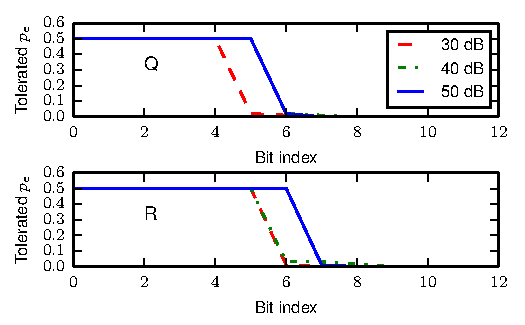
\includegraphics[width=.5\textwidth]{figs/metrics_qr}
  \caption{Tolerable imprecision of a QR decomposition, part of a 8x8 MIMO zero-forcing equalizer, for different signal qualities and a target BER=$0.01$}
  \label{fig:metrics_qr}
\end{figure}
\begin{figure}[htb]
  \centering
  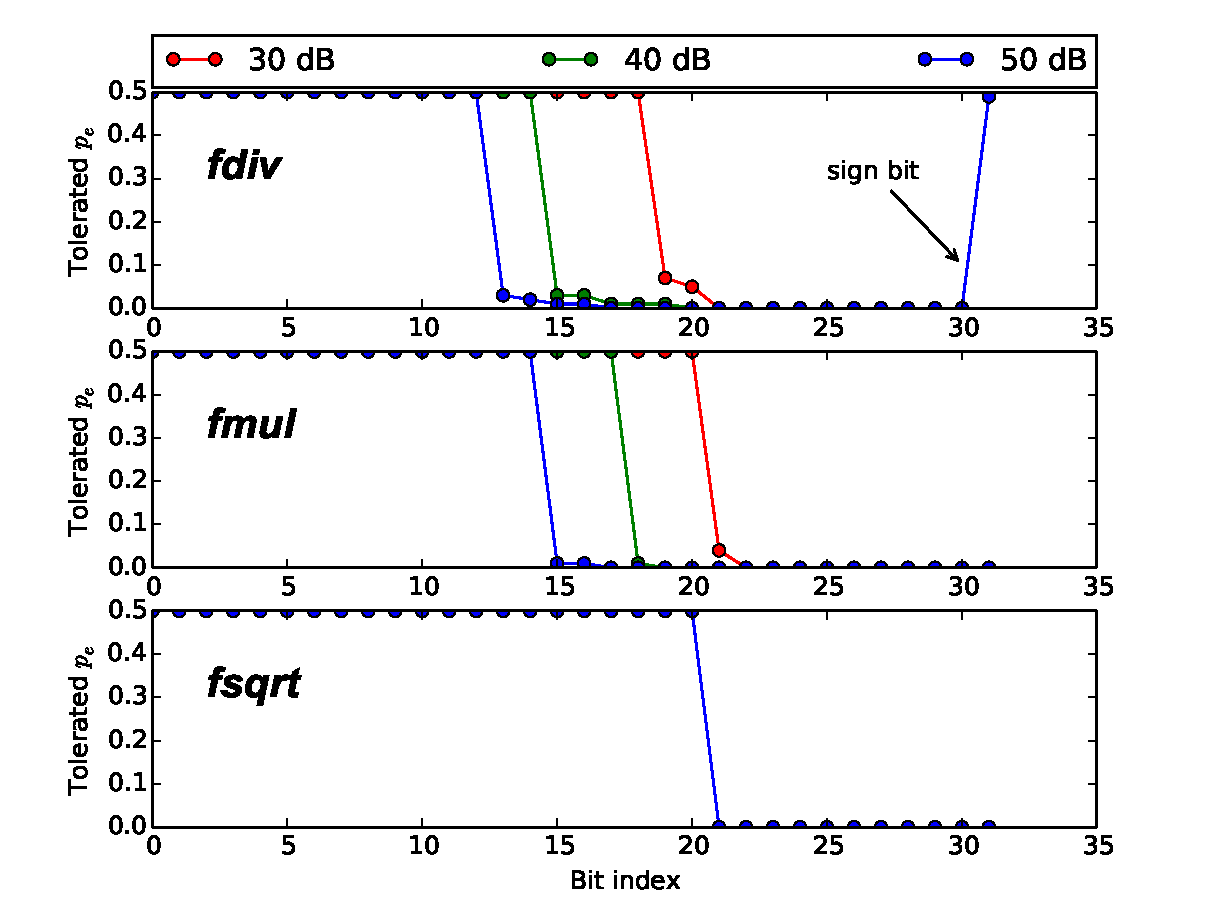
\includegraphics[width=.5\textwidth]{figs/metrics_sobel}
  \caption{Tolerable imprecision of a \emph{sobel} filter for different target qualities (PSNR)}
  \label{fig:metrics_sobel}
\end{figure}


\subsection{Approximation of Sequential Circuits}
% Hier keine Figures, verweis auf exp. results
\hl{algorithm, warum keine optimierung}
\subsubsection{Data-path Separation}
\subsubsection{High Variance Registers}
\subsubsection{Coarse-grained Approximation}
\subsubsection{Fine-grained Approximation}


















\section{Experimental Results}
\hl{Explain Circuit}\\
\begin{tabular} {| l | l | c | c |}
\hline
Name & Description & Gates & Flip-flops \\
\hline\hline
FIR & 16-tap FIR filter & xx & xx \\
IIR & 8-tap IIR filter & xx &xx \\
DCT4 & 4-input DCT & xx & xx \\
DCT8 & 8-Input DCT & xx & xx \\
fpu100 & 32-bit floating point unit & xx & xx \\
QR & QR decomposition & xx & xx \\
vitdec & Viterbi decoder (131,81) & xx & xx \\
\hline
\end{tabular}
\subsection{FPGA target}
\hl{power/area table}
\subsection{ASIC target}
\hl{power area table}














\section{Conclusion}






\section*{Acknowledgment}





% trigger a \newpage just before the given reference
% number - used to balance the columns on the last page
% adjust value as needed - may need to be readjusted if
% the document is modified later
%\IEEEtriggeratref{8}
% The "triggered" command can be changed if desired:
%\IEEEtriggercmd{\enlargethispage{-5in}}

% references section
\bibliographystyle{IEEEtran}
\bibliography{IEEEabrv,islped}





% that's all folks
\end{document}


